% Created by tikzDevice version 0.7.0 on 2014-09-22 18:04:38
% !TEX encoding = UTF-8 Unicode
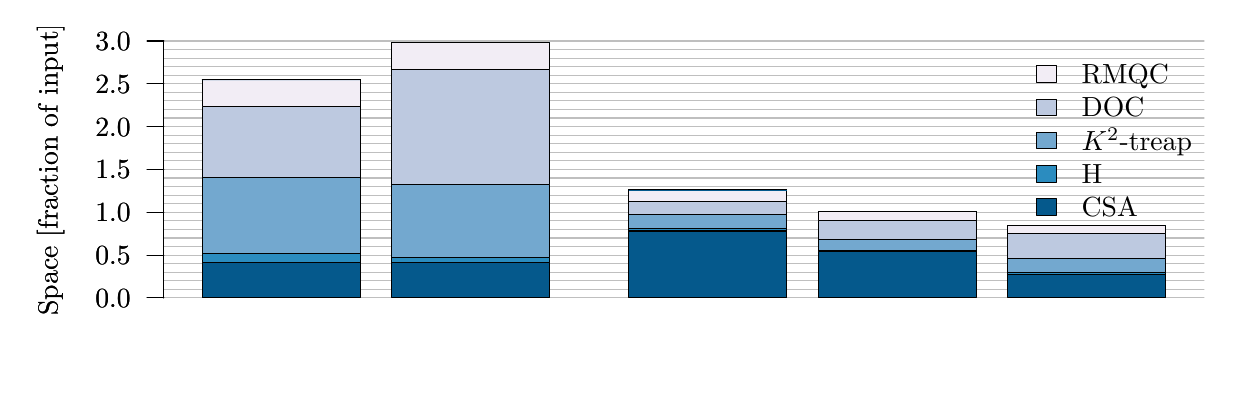
\begin{tikzpicture}[x=1pt,y=1pt]
\definecolor[named]{fillColor}{rgb}{1.00,1.00,1.00}
\path[use as bounding box,fill=fillColor,fill opacity=0.00] (0,0) rectangle (426.39,122.86);
\begin{scope}
\path[clip] (  0.00,  0.00) rectangle (426.39,122.86);
\definecolor[named]{drawColor}{rgb}{0.00,0.00,0.00}
\definecolor[named]{fillColor}{rgb}{0.02,0.35,0.55}

\path[draw=drawColor,line width= 0.4pt,line join=round,line cap=round,fill=fillColor] ( 63.13, 25.20) rectangle (120.20, 38.16);
\definecolor[named]{fillColor}{rgb}{0.17,0.55,0.75}

\path[draw=drawColor,line width= 0.4pt,line join=round,line cap=round,fill=fillColor] ( 63.13, 38.16) rectangle (120.20, 41.40);
\definecolor[named]{fillColor}{rgb}{0.45,0.66,0.81}

\path[draw=drawColor,line width= 0.4pt,line join=round,line cap=round,fill=fillColor] ( 63.13, 41.40) rectangle (120.20, 68.87);
\definecolor[named]{fillColor}{rgb}{0.74,0.79,0.88}

\path[draw=drawColor,line width= 0.4pt,line join=round,line cap=round,fill=fillColor] ( 63.13, 68.87) rectangle (120.20, 94.24);
\definecolor[named]{fillColor}{rgb}{0.95,0.93,0.96}

\path[draw=drawColor,line width= 0.4pt,line join=round,line cap=round,fill=fillColor] ( 63.13, 94.24) rectangle (120.20,104.09);
\definecolor[named]{fillColor}{rgb}{0.02,0.35,0.55}

\path[draw=drawColor,line width= 0.4pt,line join=round,line cap=round,fill=fillColor] ( 63.13,104.09) rectangle (120.20,104.09);

\path[draw=drawColor,line width= 0.4pt,line join=round,line cap=round,fill=fillColor] (131.61, 25.20) rectangle (188.68, 37.99);
\definecolor[named]{fillColor}{rgb}{0.17,0.55,0.75}

\path[draw=drawColor,line width= 0.4pt,line join=round,line cap=round,fill=fillColor] (131.61, 37.99) rectangle (188.68, 39.72);
\definecolor[named]{fillColor}{rgb}{0.45,0.66,0.81}

\path[draw=drawColor,line width= 0.4pt,line join=round,line cap=round,fill=fillColor] (131.61, 39.72) rectangle (188.68, 66.07);
\definecolor[named]{fillColor}{rgb}{0.74,0.79,0.88}

\path[draw=drawColor,line width= 0.4pt,line join=round,line cap=round,fill=fillColor] (131.61, 66.07) rectangle (188.68,107.62);
\definecolor[named]{fillColor}{rgb}{0.95,0.93,0.96}

\path[draw=drawColor,line width= 0.4pt,line join=round,line cap=round,fill=fillColor] (131.61,107.62) rectangle (188.68,117.51);
\definecolor[named]{fillColor}{rgb}{0.02,0.35,0.55}

\path[draw=drawColor,line width= 0.4pt,line join=round,line cap=round,fill=fillColor] (131.61,117.51) rectangle (188.68,117.53);

\path[draw=drawColor,line width= 0.4pt,line join=round,line cap=round,fill=fillColor] (217.22, 25.20) rectangle (274.29, 49.37);
\definecolor[named]{fillColor}{rgb}{0.17,0.55,0.75}

\path[draw=drawColor,line width= 0.4pt,line join=round,line cap=round,fill=fillColor] (217.22, 49.37) rectangle (274.29, 50.35);
\definecolor[named]{fillColor}{rgb}{0.45,0.66,0.81}

\path[draw=drawColor,line width= 0.4pt,line join=round,line cap=round,fill=fillColor] (217.22, 50.35) rectangle (274.29, 55.37);
\definecolor[named]{fillColor}{rgb}{0.74,0.79,0.88}

\path[draw=drawColor,line width= 0.4pt,line join=round,line cap=round,fill=fillColor] (217.22, 55.37) rectangle (274.29, 60.17);
\definecolor[named]{fillColor}{rgb}{0.95,0.93,0.96}

\path[draw=drawColor,line width= 0.4pt,line join=round,line cap=round,fill=fillColor] (217.22, 60.17) rectangle (274.29, 64.31);
\definecolor[named]{fillColor}{rgb}{0.02,0.35,0.55}

\path[draw=drawColor,line width= 0.4pt,line join=round,line cap=round,fill=fillColor] (217.22, 64.31) rectangle (274.29, 64.32);

\path[draw=drawColor,line width= 0.4pt,line join=round,line cap=round,fill=fillColor] (285.71, 25.20) rectangle (342.78, 41.89);
\definecolor[named]{fillColor}{rgb}{0.17,0.55,0.75}

\path[draw=drawColor,line width= 0.4pt,line join=round,line cap=round,fill=fillColor] (285.71, 41.89) rectangle (342.78, 42.38);
\definecolor[named]{fillColor}{rgb}{0.45,0.66,0.81}

\path[draw=drawColor,line width= 0.4pt,line join=round,line cap=round,fill=fillColor] (285.71, 42.38) rectangle (342.78, 46.44);
\definecolor[named]{fillColor}{rgb}{0.74,0.79,0.88}

\path[draw=drawColor,line width= 0.4pt,line join=round,line cap=round,fill=fillColor] (285.71, 46.44) rectangle (342.78, 53.04);
\definecolor[named]{fillColor}{rgb}{0.95,0.93,0.96}

\path[draw=drawColor,line width= 0.4pt,line join=round,line cap=round,fill=fillColor] (285.71, 53.04) rectangle (342.78, 56.46);
\definecolor[named]{fillColor}{rgb}{0.02,0.35,0.55}

\path[draw=drawColor,line width= 0.4pt,line join=round,line cap=round,fill=fillColor] (285.71, 56.46) rectangle (342.78, 56.50);

\path[draw=drawColor,line width= 0.4pt,line join=round,line cap=round,fill=fillColor] (354.19, 25.20) rectangle (411.27, 33.70);
\definecolor[named]{fillColor}{rgb}{0.17,0.55,0.75}

\path[draw=drawColor,line width= 0.4pt,line join=round,line cap=round,fill=fillColor] (354.19, 33.70) rectangle (411.27, 34.32);
\definecolor[named]{fillColor}{rgb}{0.45,0.66,0.81}

\path[draw=drawColor,line width= 0.4pt,line join=round,line cap=round,fill=fillColor] (354.19, 34.32) rectangle (411.27, 39.35);
\definecolor[named]{fillColor}{rgb}{0.74,0.79,0.88}

\path[draw=drawColor,line width= 0.4pt,line join=round,line cap=round,fill=fillColor] (354.19, 39.35) rectangle (411.27, 48.47);
\definecolor[named]{fillColor}{rgb}{0.95,0.93,0.96}

\path[draw=drawColor,line width= 0.4pt,line join=round,line cap=round,fill=fillColor] (354.19, 48.47) rectangle (411.27, 51.50);
\definecolor[named]{fillColor}{rgb}{0.02,0.35,0.55}

\path[draw=drawColor,line width= 0.4pt,line join=round,line cap=round,fill=fillColor] (354.19, 51.50) rectangle (411.27, 51.52);
\end{scope}
\begin{scope}
\path[clip] (  0.00,  0.00) rectangle (426.39,122.86);
\definecolor[named]{drawColor}{rgb}{0.00,0.00,0.00}

\node[text=drawColor,anchor=base,inner sep=0pt, outer sep=0pt, scale=  1.00] at ( 91.66,  3.60) {\ENWIKISML};

\node[text=drawColor,anchor=base,inner sep=0pt, outer sep=0pt, scale=  1.00] at (160.15,  3.60) {\ENWIKIBIG};

\node[text=drawColor,anchor=base,inner sep=0pt, outer sep=0pt, scale=  1.00] at (245.76,  3.60) {\ENWIKISMLINT};

\node[text=drawColor,anchor=base,inner sep=0pt, outer sep=0pt, scale=  1.00] at (314.24,  3.60) {\ENWIKIBIGINT};

\node[text=drawColor,anchor=base,inner sep=0pt, outer sep=0pt, scale=  1.00] at (382.73,  3.60) {\GOVII};
\end{scope}
\begin{scope}
\path[clip] (  0.00,  0.00) rectangle (426.39,122.86);
\definecolor[named]{drawColor}{rgb}{0.00,0.00,0.00}

\node[text=drawColor,rotate= 90.00,anchor=base,inner sep=0pt, outer sep=0pt, scale=  1.00] at ( 10.80, 71.63) {Space [fraction of input]};
\end{scope}
\begin{scope}
\path[clip] (  0.00,  0.00) rectangle (426.39,122.86);
\definecolor[named]{drawColor}{rgb}{0.00,0.00,0.00}

\path[draw=drawColor,line width= 0.4pt,line join=round,line cap=round] ( 49.20, 25.20) -- ( 49.20,118.06);

\path[draw=drawColor,line width= 0.4pt,line join=round,line cap=round] ( 49.20, 25.20) -- ( 43.20, 25.20);

\path[draw=drawColor,line width= 0.4pt,line join=round,line cap=round] ( 49.20, 40.68) -- ( 43.20, 40.68);

\path[draw=drawColor,line width= 0.4pt,line join=round,line cap=round] ( 49.20, 56.15) -- ( 43.20, 56.15);

\path[draw=drawColor,line width= 0.4pt,line join=round,line cap=round] ( 49.20, 71.63) -- ( 43.20, 71.63);

\path[draw=drawColor,line width= 0.4pt,line join=round,line cap=round] ( 49.20, 87.11) -- ( 43.20, 87.11);

\path[draw=drawColor,line width= 0.4pt,line join=round,line cap=round] ( 49.20,102.58) -- ( 43.20,102.58);

\path[draw=drawColor,line width= 0.4pt,line join=round,line cap=round] ( 49.20,118.06) -- ( 43.20,118.06);

\node[text=drawColor,anchor=base east,inner sep=0pt, outer sep=0pt, scale=  1.00] at ( 37.20, 21.76) {0.0};

\node[text=drawColor,anchor=base east,inner sep=0pt, outer sep=0pt, scale=  1.00] at ( 37.20, 37.23) {0.5};

\node[text=drawColor,anchor=base east,inner sep=0pt, outer sep=0pt, scale=  1.00] at ( 37.20, 52.71) {1.0};

\node[text=drawColor,anchor=base east,inner sep=0pt, outer sep=0pt, scale=  1.00] at ( 37.20, 68.19) {1.5};

\node[text=drawColor,anchor=base east,inner sep=0pt, outer sep=0pt, scale=  1.00] at ( 37.20, 83.66) {2.0};

\node[text=drawColor,anchor=base east,inner sep=0pt, outer sep=0pt, scale=  1.00] at ( 37.20, 99.14) {2.5};

\node[text=drawColor,anchor=base east,inner sep=0pt, outer sep=0pt, scale=  1.00] at ( 37.20,114.62) {3.0};
\end{scope}
\begin{scope}
\path[clip] ( 49.20, 25.20) rectangle (425.19,118.06);
\definecolor[named]{drawColor}{rgb}{0.75,0.75,0.75}

\path[draw=drawColor,line width= 0.4pt,line join=round,line cap=round] ( 49.20, 25.20) -- (425.19, 25.20);

\path[draw=drawColor,line width= 0.4pt,line join=round,line cap=round] ( 49.20, 28.30) -- (425.19, 28.30);

\path[draw=drawColor,line width= 0.4pt,line join=round,line cap=round] ( 49.20, 31.39) -- (425.19, 31.39);

\path[draw=drawColor,line width= 0.4pt,line join=round,line cap=round] ( 49.20, 34.49) -- (425.19, 34.49);

\path[draw=drawColor,line width= 0.4pt,line join=round,line cap=round] ( 49.20, 37.58) -- (425.19, 37.58);

\path[draw=drawColor,line width= 0.4pt,line join=round,line cap=round] ( 49.20, 40.68) -- (425.19, 40.68);

\path[draw=drawColor,line width= 0.4pt,line join=round,line cap=round] ( 49.20, 43.77) -- (425.19, 43.77);

\path[draw=drawColor,line width= 0.4pt,line join=round,line cap=round] ( 49.20, 46.87) -- (425.19, 46.87);

\path[draw=drawColor,line width= 0.4pt,line join=round,line cap=round] ( 49.20, 49.96) -- (425.19, 49.96);

\path[draw=drawColor,line width= 0.4pt,line join=round,line cap=round] ( 49.20, 53.06) -- (425.19, 53.06);

\path[draw=drawColor,line width= 0.4pt,line join=round,line cap=round] ( 49.20, 56.15) -- (425.19, 56.15);

\path[draw=drawColor,line width= 0.4pt,line join=round,line cap=round] ( 49.20, 59.25) -- (425.19, 59.25);

\path[draw=drawColor,line width= 0.4pt,line join=round,line cap=round] ( 49.20, 62.34) -- (425.19, 62.34);

\path[draw=drawColor,line width= 0.4pt,line join=round,line cap=round] ( 49.20, 65.44) -- (425.19, 65.44);

\path[draw=drawColor,line width= 0.4pt,line join=round,line cap=round] ( 49.20, 68.53) -- (425.19, 68.53);

\path[draw=drawColor,line width= 0.4pt,line join=round,line cap=round] ( 49.20, 71.63) -- (425.19, 71.63);

\path[draw=drawColor,line width= 0.4pt,line join=round,line cap=round] ( 49.20, 74.72) -- (425.19, 74.72);

\path[draw=drawColor,line width= 0.4pt,line join=round,line cap=round] ( 49.20, 77.82) -- (425.19, 77.82);

\path[draw=drawColor,line width= 0.4pt,line join=round,line cap=round] ( 49.20, 80.92) -- (425.19, 80.92);

\path[draw=drawColor,line width= 0.4pt,line join=round,line cap=round] ( 49.20, 84.01) -- (425.19, 84.01);

\path[draw=drawColor,line width= 0.4pt,line join=round,line cap=round] ( 49.20, 87.11) -- (425.19, 87.11);

\path[draw=drawColor,line width= 0.4pt,line join=round,line cap=round] ( 49.20, 90.20) -- (425.19, 90.20);

\path[draw=drawColor,line width= 0.4pt,line join=round,line cap=round] ( 49.20, 93.30) -- (425.19, 93.30);

\path[draw=drawColor,line width= 0.4pt,line join=round,line cap=round] ( 49.20, 96.39) -- (425.19, 96.39);

\path[draw=drawColor,line width= 0.4pt,line join=round,line cap=round] ( 49.20, 99.49) -- (425.19, 99.49);

\path[draw=drawColor,line width= 0.4pt,line join=round,line cap=round] ( 49.20,102.58) -- (425.19,102.58);

\path[draw=drawColor,line width= 0.4pt,line join=round,line cap=round] ( 49.20,105.68) -- (425.19,105.68);

\path[draw=drawColor,line width= 0.4pt,line join=round,line cap=round] ( 49.20,108.77) -- (425.19,108.77);

\path[draw=drawColor,line width= 0.4pt,line join=round,line cap=round] ( 49.20,111.87) -- (425.19,111.87);

\path[draw=drawColor,line width= 0.4pt,line join=round,line cap=round] ( 49.20,114.96) -- (425.19,114.96);

\path[draw=drawColor,line width= 0.4pt,line join=round,line cap=round] ( 49.20,118.06) -- (425.19,118.06);
\end{scope}
\begin{scope}
\path[clip] (  0.00,  0.00) rectangle (426.39,122.86);
\definecolor[named]{drawColor}{rgb}{0.00,0.00,0.00}
\definecolor[named]{fillColor}{rgb}{0.02,0.35,0.55}

\path[draw=drawColor,line width= 0.4pt,line join=round,line cap=round,fill=fillColor] ( 63.13, 25.20) rectangle (120.20, 38.16);
\definecolor[named]{fillColor}{rgb}{0.17,0.55,0.75}

\path[draw=drawColor,line width= 0.4pt,line join=round,line cap=round,fill=fillColor] ( 63.13, 38.16) rectangle (120.20, 41.40);
\definecolor[named]{fillColor}{rgb}{0.45,0.66,0.81}

\path[draw=drawColor,line width= 0.4pt,line join=round,line cap=round,fill=fillColor] ( 63.13, 41.40) rectangle (120.20, 68.87);
\definecolor[named]{fillColor}{rgb}{0.74,0.79,0.88}

\path[draw=drawColor,line width= 0.4pt,line join=round,line cap=round,fill=fillColor] ( 63.13, 68.87) rectangle (120.20, 94.24);
\definecolor[named]{fillColor}{rgb}{0.95,0.93,0.96}

\path[draw=drawColor,line width= 0.4pt,line join=round,line cap=round,fill=fillColor] ( 63.13, 94.24) rectangle (120.20,104.09);
\definecolor[named]{fillColor}{rgb}{0.02,0.35,0.55}

\path[draw=drawColor,line width= 0.4pt,line join=round,line cap=round,fill=fillColor] ( 63.13,104.09) rectangle (120.20,104.09);

\path[draw=drawColor,line width= 0.4pt,line join=round,line cap=round,fill=fillColor] (131.61, 25.20) rectangle (188.68, 37.99);
\definecolor[named]{fillColor}{rgb}{0.17,0.55,0.75}

\path[draw=drawColor,line width= 0.4pt,line join=round,line cap=round,fill=fillColor] (131.61, 37.99) rectangle (188.68, 39.72);
\definecolor[named]{fillColor}{rgb}{0.45,0.66,0.81}

\path[draw=drawColor,line width= 0.4pt,line join=round,line cap=round,fill=fillColor] (131.61, 39.72) rectangle (188.68, 66.07);
\definecolor[named]{fillColor}{rgb}{0.74,0.79,0.88}

\path[draw=drawColor,line width= 0.4pt,line join=round,line cap=round,fill=fillColor] (131.61, 66.07) rectangle (188.68,107.62);
\definecolor[named]{fillColor}{rgb}{0.95,0.93,0.96}

\path[draw=drawColor,line width= 0.4pt,line join=round,line cap=round,fill=fillColor] (131.61,107.62) rectangle (188.68,117.51);
\definecolor[named]{fillColor}{rgb}{0.02,0.35,0.55}

\path[draw=drawColor,line width= 0.4pt,line join=round,line cap=round,fill=fillColor] (131.61,117.51) rectangle (188.68,117.53);

\path[draw=drawColor,line width= 0.4pt,line join=round,line cap=round,fill=fillColor] (217.22, 25.20) rectangle (274.29, 49.37);
\definecolor[named]{fillColor}{rgb}{0.17,0.55,0.75}

\path[draw=drawColor,line width= 0.4pt,line join=round,line cap=round,fill=fillColor] (217.22, 49.37) rectangle (274.29, 50.35);
\definecolor[named]{fillColor}{rgb}{0.45,0.66,0.81}

\path[draw=drawColor,line width= 0.4pt,line join=round,line cap=round,fill=fillColor] (217.22, 50.35) rectangle (274.29, 55.37);
\definecolor[named]{fillColor}{rgb}{0.74,0.79,0.88}

\path[draw=drawColor,line width= 0.4pt,line join=round,line cap=round,fill=fillColor] (217.22, 55.37) rectangle (274.29, 60.17);
\definecolor[named]{fillColor}{rgb}{0.95,0.93,0.96}

\path[draw=drawColor,line width= 0.4pt,line join=round,line cap=round,fill=fillColor] (217.22, 60.17) rectangle (274.29, 64.31);
\definecolor[named]{fillColor}{rgb}{0.02,0.35,0.55}

\path[draw=drawColor,line width= 0.4pt,line join=round,line cap=round,fill=fillColor] (217.22, 64.31) rectangle (274.29, 64.32);

\path[draw=drawColor,line width= 0.4pt,line join=round,line cap=round,fill=fillColor] (285.71, 25.20) rectangle (342.78, 41.89);
\definecolor[named]{fillColor}{rgb}{0.17,0.55,0.75}

\path[draw=drawColor,line width= 0.4pt,line join=round,line cap=round,fill=fillColor] (285.71, 41.89) rectangle (342.78, 42.38);
\definecolor[named]{fillColor}{rgb}{0.45,0.66,0.81}

\path[draw=drawColor,line width= 0.4pt,line join=round,line cap=round,fill=fillColor] (285.71, 42.38) rectangle (342.78, 46.44);
\definecolor[named]{fillColor}{rgb}{0.74,0.79,0.88}

\path[draw=drawColor,line width= 0.4pt,line join=round,line cap=round,fill=fillColor] (285.71, 46.44) rectangle (342.78, 53.04);
\definecolor[named]{fillColor}{rgb}{0.95,0.93,0.96}

\path[draw=drawColor,line width= 0.4pt,line join=round,line cap=round,fill=fillColor] (285.71, 53.04) rectangle (342.78, 56.46);
\definecolor[named]{fillColor}{rgb}{0.02,0.35,0.55}

\path[draw=drawColor,line width= 0.4pt,line join=round,line cap=round,fill=fillColor] (285.71, 56.46) rectangle (342.78, 56.50);

\path[draw=drawColor,line width= 0.4pt,line join=round,line cap=round,fill=fillColor] (354.19, 25.20) rectangle (411.27, 33.70);
\definecolor[named]{fillColor}{rgb}{0.17,0.55,0.75}

\path[draw=drawColor,line width= 0.4pt,line join=round,line cap=round,fill=fillColor] (354.19, 33.70) rectangle (411.27, 34.32);
\definecolor[named]{fillColor}{rgb}{0.45,0.66,0.81}

\path[draw=drawColor,line width= 0.4pt,line join=round,line cap=round,fill=fillColor] (354.19, 34.32) rectangle (411.27, 39.35);
\definecolor[named]{fillColor}{rgb}{0.74,0.79,0.88}

\path[draw=drawColor,line width= 0.4pt,line join=round,line cap=round,fill=fillColor] (354.19, 39.35) rectangle (411.27, 48.47);
\definecolor[named]{fillColor}{rgb}{0.95,0.93,0.96}

\path[draw=drawColor,line width= 0.4pt,line join=round,line cap=round,fill=fillColor] (354.19, 48.47) rectangle (411.27, 51.50);
\definecolor[named]{fillColor}{rgb}{0.02,0.35,0.55}

\path[draw=drawColor,line width= 0.4pt,line join=round,line cap=round,fill=fillColor] (354.19, 51.50) rectangle (411.27, 51.52);
\end{scope}
\begin{scope}
\path[clip] (  0.00,  0.00) rectangle (426.39,122.86);
\definecolor[named]{drawColor}{rgb}{0.00,0.00,0.00}

\node[text=drawColor,anchor=base,inner sep=0pt, outer sep=0pt, scale=  1.00] at ( 91.66,  3.60) {\ENWIKISML};

\node[text=drawColor,anchor=base,inner sep=0pt, outer sep=0pt, scale=  1.00] at (160.15,  3.60) {\ENWIKIBIG};

\node[text=drawColor,anchor=base,inner sep=0pt, outer sep=0pt, scale=  1.00] at (245.76,  3.60) {\ENWIKISMLINT};

\node[text=drawColor,anchor=base,inner sep=0pt, outer sep=0pt, scale=  1.00] at (314.24,  3.60) {\ENWIKIBIGINT};

\node[text=drawColor,anchor=base,inner sep=0pt, outer sep=0pt, scale=  1.00] at (382.73,  3.60) {\GOVII};
\end{scope}
\begin{scope}
\path[clip] (  0.00,  0.00) rectangle (426.39,122.86);
\definecolor[named]{drawColor}{rgb}{0.00,0.00,0.00}

\node[text=drawColor,rotate= 90.00,anchor=base,inner sep=0pt, outer sep=0pt, scale=  1.00] at ( 10.80, 71.63) {Space [fraction of input]};
\end{scope}
\begin{scope}
\path[clip] (  0.00,  0.00) rectangle (426.39,122.86);
\definecolor[named]{drawColor}{rgb}{0.00,0.00,0.00}

\path[draw=drawColor,line width= 0.4pt,line join=round,line cap=round] ( 49.20, 25.20) -- ( 49.20,118.06);

\path[draw=drawColor,line width= 0.4pt,line join=round,line cap=round] ( 49.20, 25.20) -- ( 43.20, 25.20);

\path[draw=drawColor,line width= 0.4pt,line join=round,line cap=round] ( 49.20, 40.68) -- ( 43.20, 40.68);

\path[draw=drawColor,line width= 0.4pt,line join=round,line cap=round] ( 49.20, 56.15) -- ( 43.20, 56.15);

\path[draw=drawColor,line width= 0.4pt,line join=round,line cap=round] ( 49.20, 71.63) -- ( 43.20, 71.63);

\path[draw=drawColor,line width= 0.4pt,line join=round,line cap=round] ( 49.20, 87.11) -- ( 43.20, 87.11);

\path[draw=drawColor,line width= 0.4pt,line join=round,line cap=round] ( 49.20,102.58) -- ( 43.20,102.58);

\path[draw=drawColor,line width= 0.4pt,line join=round,line cap=round] ( 49.20,118.06) -- ( 43.20,118.06);

\node[text=drawColor,anchor=base east,inner sep=0pt, outer sep=0pt, scale=  1.00] at ( 37.20, 21.76) {0.0};

\node[text=drawColor,anchor=base east,inner sep=0pt, outer sep=0pt, scale=  1.00] at ( 37.20, 37.23) {0.5};

\node[text=drawColor,anchor=base east,inner sep=0pt, outer sep=0pt, scale=  1.00] at ( 37.20, 52.71) {1.0};

\node[text=drawColor,anchor=base east,inner sep=0pt, outer sep=0pt, scale=  1.00] at ( 37.20, 68.19) {1.5};

\node[text=drawColor,anchor=base east,inner sep=0pt, outer sep=0pt, scale=  1.00] at ( 37.20, 83.66) {2.0};

\node[text=drawColor,anchor=base east,inner sep=0pt, outer sep=0pt, scale=  1.00] at ( 37.20, 99.14) {2.5};

\node[text=drawColor,anchor=base east,inner sep=0pt, outer sep=0pt, scale=  1.00] at ( 37.20,114.62) {3.0};
\end{scope}
\begin{scope}
\path[clip] ( 49.20, 25.20) rectangle (425.19,118.06);
\definecolor[named]{drawColor}{rgb}{0.00,0.00,0.00}
\definecolor[named]{fillColor}{rgb}{0.95,0.93,0.96}

\path[draw=drawColor,line width= 0.4pt,line join=round,line cap=round,fill=fillColor] (364.67,109.06) rectangle (371.87,103.06);
\definecolor[named]{fillColor}{rgb}{0.74,0.79,0.88}

\path[draw=drawColor,line width= 0.4pt,line join=round,line cap=round,fill=fillColor] (364.67, 97.06) rectangle (371.87, 91.06);
\definecolor[named]{fillColor}{rgb}{0.45,0.66,0.81}

\path[draw=drawColor,line width= 0.4pt,line join=round,line cap=round,fill=fillColor] (364.67, 85.06) rectangle (371.87, 79.06);
\definecolor[named]{fillColor}{rgb}{0.17,0.55,0.75}

\path[draw=drawColor,line width= 0.4pt,line join=round,line cap=round,fill=fillColor] (364.67, 73.06) rectangle (371.87, 67.06);
\definecolor[named]{fillColor}{rgb}{0.02,0.35,0.55}

\path[draw=drawColor,line width= 0.4pt,line join=round,line cap=round,fill=fillColor] (364.67, 61.06) rectangle (371.87, 55.06);

\node[text=drawColor,anchor=base west,inner sep=0pt, outer sep=0pt, scale=  1.00] at (380.87,102.62) {RMQC};

\node[text=drawColor,anchor=base west,inner sep=0pt, outer sep=0pt, scale=  1.00] at (380.87, 90.62) {DOC};

\node[text=drawColor,anchor=base west,inner sep=0pt, outer sep=0pt, scale=  1.00] at (380.87, 78.62) {$K^2$-treap};

\node[text=drawColor,anchor=base west,inner sep=0pt, outer sep=0pt, scale=  1.00] at (380.87, 66.62) {H};

\node[text=drawColor,anchor=base west,inner sep=0pt, outer sep=0pt, scale=  1.00] at (380.87, 54.62) {CSA};
\end{scope}
\end{tikzpicture}
